\documentclass[12pt]{article}
\scrollmode
\thispagestyle{empty}
%\usepackage{latexsym}
\usepackage{fancyhdr}
\def\myfooter{\vfill{\footnotesize\noindent\copyright\ 2016, Manfred Kerber, School of Computer Science, University of Birmingham}}
%\usepackage{colordvi}
\usepackage{url}
%\usepackage{bbm}
%\usepackage{verbatim}
%%%%%%%%%
%\usepackage{listings}
%\lstloadlanguages{Java,csh}
%\lstset{basicstyle=\ttfamily\normalsize,columns=fixed,breaklines=true,language=Java,showstringspaces=false}
%\lstMakeShortInline|

%%%%%%%%%%

\newif\ifslide\slidetrue
\newif\ifnotes\notesfalse
\newif\ifColour\Colourfalse
\newif\ifpdf\pdffalse
\usepackage{code}
\usepackage{epsfig}
\usepackage{a4wide}
%\usepackage{pstricks,pst-node}
%\addtolength{\textheight}{2.5cm}%{4ex}
\newcommand{\myhead}[1]{\begin{center}\large\bf #1\end{center}}
%\input{ex-macros} 
%\includeonly{linclass}
\begin{document}
\myhead{Lab lecture exercises -- 25 November 2016}

\begin{enumerate}
\item Write a class \texttt{Measure} with two field variables
  \texttt{private String description} and \texttt{private int value},
  where a value is always non-negative (e.g., this could be films with
  a rating, bank accounts with a non-negative balance, processes with
  times needed to complete them, customers and their age, and so on).
\item Assume now a variable \texttt{private ArrayList<Measure>
    measures} which collects several of these measures of the same
  type.

  Create a class \texttt{BarChart} for a visual presentation of the
  measures by creating vertical bars (see, e.g.,
  http://www.mathsisfun.com/data/bar-graphs.html}) from a given
  \texttt{private ArrayList<Measure> measures}.

  To this end:
  \begin{enumerate}
  \item Compute the maximum of \texttt{measures}. If it is non-zero,
    normalize the values so that the maximal bar is represented by a
    given number of pixels such as \texttt{int yNumberOfPixels =
      400}. The panel should have a size of 800 times 500 pixels.

  \item Write a method \texttt{public static ArrayList<Measure>
      randomMeasures(int n, int low, int high)} that generates an
    ArrayList of type \texttt{Measure} with length \texttt{n} and
    random values between \texttt{low} and \texttt{high}.

  \item For a ``short'' ArrayList (i.e., size less than or equal to
    10) present the bar chart by bars of width \texttt{30}
    pixel and the empty space between two bars by \texttt{10} pixels.
\begin{center}
  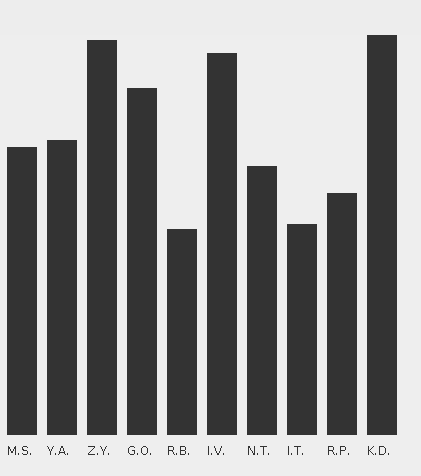
\includegraphics[width=0.2\textwidth]{bars.png}
\end{center}

\item If the ArrayList is bigger (i.e., sizes greater than 10 but less
  than or equal to 100) reduce the width of the bars and the gaps down
  to \texttt{3} and \texttt{1} for an ArrayList of size 100; and to
  something in between \texttt{3} and \texttt{30} for the width of the
  bars (in between \texttt{1} and \texttt{10} for the gaps) for not
  quite so long ArrayLists.

  \item For ArrayLists with sizes less than or equal to 30 display a
    \texttt{description} below the bars.

  \item If the ArrayList is even bigger (i.e., greater than 100
    elements, but less than or equal to 600 pixels) use the
    \texttt{fillPolygon} method to display the values.

  \item If the ArrayList is even bigger (greater than 600 pixels)
    print just out a warning that the ArrayList cannot be displayed.
  \end{enumerate}


%\vfill
%\hfill p.t.o.
%\newpage
\end{enumerate}

\myfooter
\end{document}

%%% Local Variables: 
%%% mode: latex
%%% TeX-master: t
%%% End: 
